\chapter{Herramienta gráfica de experimentación}

\section{Necesidad de este tipo de herramientas}
Necesitamos una interfaz gráfica (GUI) para la ejecución continua de algoritmos. Con ligeras variaciones, pero siempre presentando los resultados de forma inmediata y eficaz.

El patrón que mejor se nos ajusta es \textit{Feature, Search and Browse} \cite{tidwell2010designing}, porque podemos tener tanto los parámetros como el resultado de su ejecución a la vista, al mismo tiempo.
\begin{figure}[H]
\centering
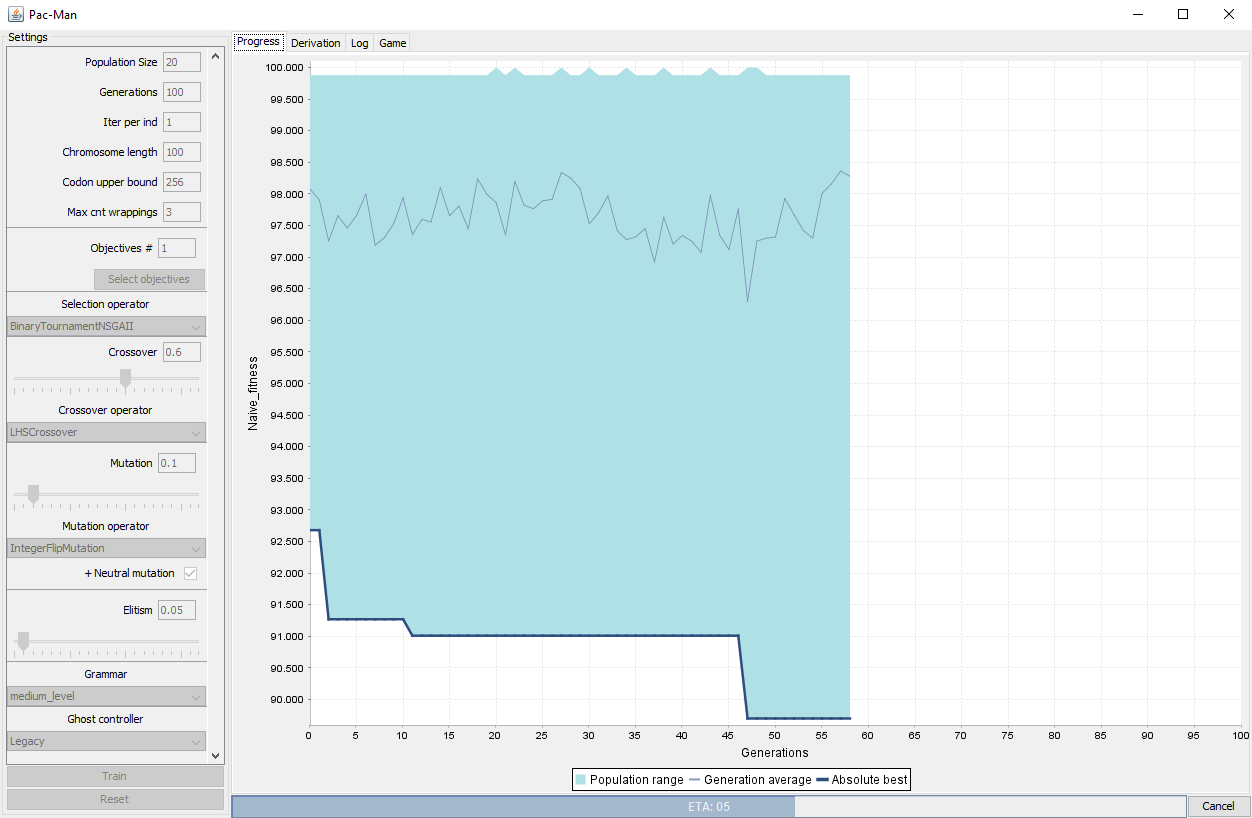
\includegraphics[width=\textwidth]{gui/portada}
\end{figure}

\section{Panel de ajustes del experimento}
A la izquierda tenemos el panel de los ajustes. Aquí se pueden modificar parámetros tanto del algoritmo evolutivo como de Pac-Man. Haremos una explicación por partes.
 
En la parte inferior izquierda pueden verse dos botones. \textit{Train} comienza la ejecución del algoritmo con los parámetros establecidos, mientras que \textit{Reset} revierte todos los parámetros a su valor por defecto.
\begin{figure}[H]
\centering

\includegraphics[width=6cm]{gui/train-reset}
\end{figure}

Una vez que finaliza la ejecución del algoritmo puede verse que aparece un botón más.
\begin{figure}[H]
\centering
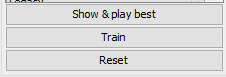
\includegraphics[width=6cm]{gui/train-reset-showplay}
\end{figure}

\textit{Show \& play best} es un atajo que cambia a la pestaña donde se ejecuta Pac-Man de manera visual, copia el fenotipo del mejor individuo en la ventana de edición y comienza la ejecución del fenotipo en el juego automáticamente.

\subsection{Parámetros del algoritmo}
Comenzando por la parte de arriba, tenemos los parámetros concretos del algoritmo de evolución gramatical.
\begin{figure}[H]
\centering
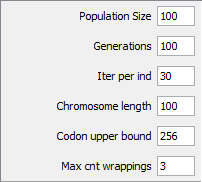
\includegraphics[width=5.5cm]{gui/parametros-algo}
\end{figure}

Con estos parámetros se pueden manejar:
\begin{itemize}
\item \textbf{\textit{Population Size}}: Tamaño de la población.

\item \textbf{\textit{Generations}}: Número de generaciones (iteraciones del algoritmo).

\item \textbf{\textit{Iter per Ind}}: Número de partidas que juega un individuo para evaluarlo.

\item \textbf{\textit{Chromosome length}}: Tamaño del cromosoma (número de codones).

\item \textbf{\textit{Codon upper bound}}: Número máximo que puede alcanzar un codón.

\item \textbf{\textit{Max cnt wrappings}}: Número máximo de \textit{wrappings} permitidos al derivar un codón.
\end{itemize}

Posteriormente tenemos el selector de objetivos del algoritmo evolutivo.
\begin{figure}[H]
\centering

\includegraphics[width=5.5cm]{gui/objetivos}
\end{figure}

Donde ya hemos visto que se puede seleccionar la combinación de los mismos que se quiera.
\begin{figure}[H]
\centering
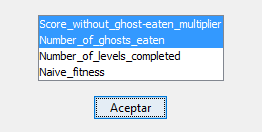
\includegraphics[width=7cm]{gui/objetivos-selector}
\end{figure}

A continuación tenemos los parámetros generales de cualquier algoritmo evolutivo: métodos de selección, operadores de cruce y operadores de mutación que se pueden seleccionar desde listas desplegables. Para el cruce y la mutación también se puede elegir la probabilidad con la que se va a aplicar el operador, la cual se puede seleccionar desde el \textit{slider} o escribir directamente en el campo de texto para mayor precisión (valores de $0$ a $1$).
\begin{figure}[H]
\centering

\includegraphics[width=5.5cm]{gui/seleccion}
\end{figure}
\begin{figure}[H]
\centering
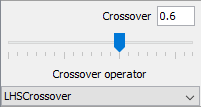
\includegraphics[width=5.5cm]{gui/cruce}
\end{figure}
\begin{figure}[H]
\centering
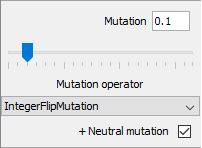
\includegraphics[width=5.5cm]{gui/mutacion}
\end{figure}

Asimismo, podemos seleccionar el porcentaje de elitismo en el algoritmo genético ya sea por \textit{slider} o campo de texto.
\begin{figure}[H]
\centering

\includegraphics[width=5.5cm]{gui/elitismo}
\end{figure}

\subsection{Parámetros de Pac-Man}
Después tenemos un selector de gramáticas que el algoritmo gramatical es capaz de usar para su evolución.
\begin{figure}[H]
\centering

\includegraphics[width=5.5cm]{gui/grammar}
\end{figure}

Por último tenemos el controlador que los fantasmas van a usar cada vez que se juegue una partida.
\begin{figure}[H]
\centering

\includegraphics[width=5.5cm]{gui/ghost-controller}
\end{figure}

\section{Panel de progreso}
\begin{figure}[H]
\centering
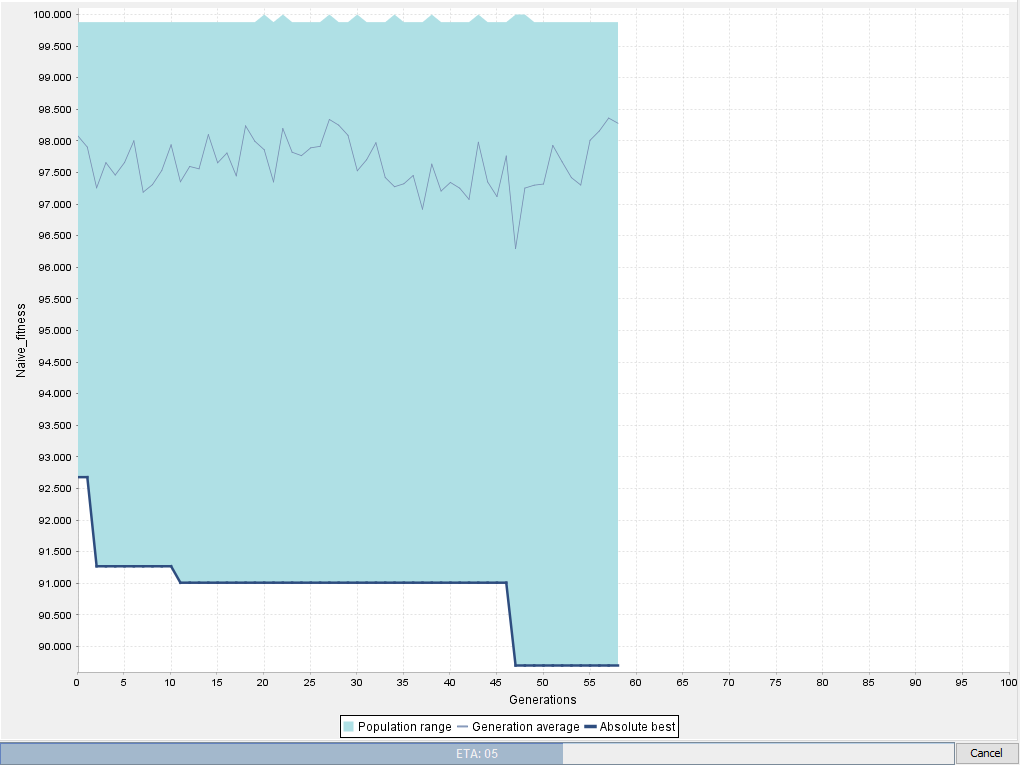
\includegraphics[width=\textwidth]{gui/progreso}
\end{figure}

Aquí vemos en tiempo real el \textit{fitness} de los individuos con cada generación, es decir, cuánto mejor se está volviendo la población. Está descendiendo porque hacemos minimización.

El eje $X$ representa el número de generaciones (iteraciones del algoritmo). El eje $Y$ son los puntos de \textit{fitness} que se están alcanzando. Si se seleccionaran dos o más objetivos, la gráfica tendría una subfigura por cada objetivo, donde se mostraría el \textit{fitness} de cada uno por separado.

La línea azul gruesa es el \textit{fitness} del mejor individuo de entre toda la población, para esa iteración del algoritmo.

La línea azul delgada indica la media del \textit{fitness} de toda la población. Con esta línea se puede discernir la puntuación global.

La franja indica el rango de \textit{fitness} en el que se mueve la población, que comprende desde el peor \textit{fitness} al mejor.

El esquema de color está inspirado en el que usa GEVA \cite{gevaGit}.

\subsection{Multiobjetivo}
También se puede visualizar el \textit{fitness} en caso de que seleccionemos más de un objetivo.
\begin{figure}[H]
\centering
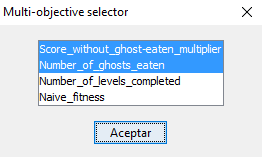
\includegraphics[width=7cm]{gui/objetivos-selector2}
\end{figure}

En ese caso se mostrarían tantas gráficas como objetivos hayamos seleccionado, teniendo cada una sus propias estadísticas para analizar la evolución de cada objetivo por separado, además de poder vislumbrar relaciones en conjunto.
\begin{figure}[H]
\centering
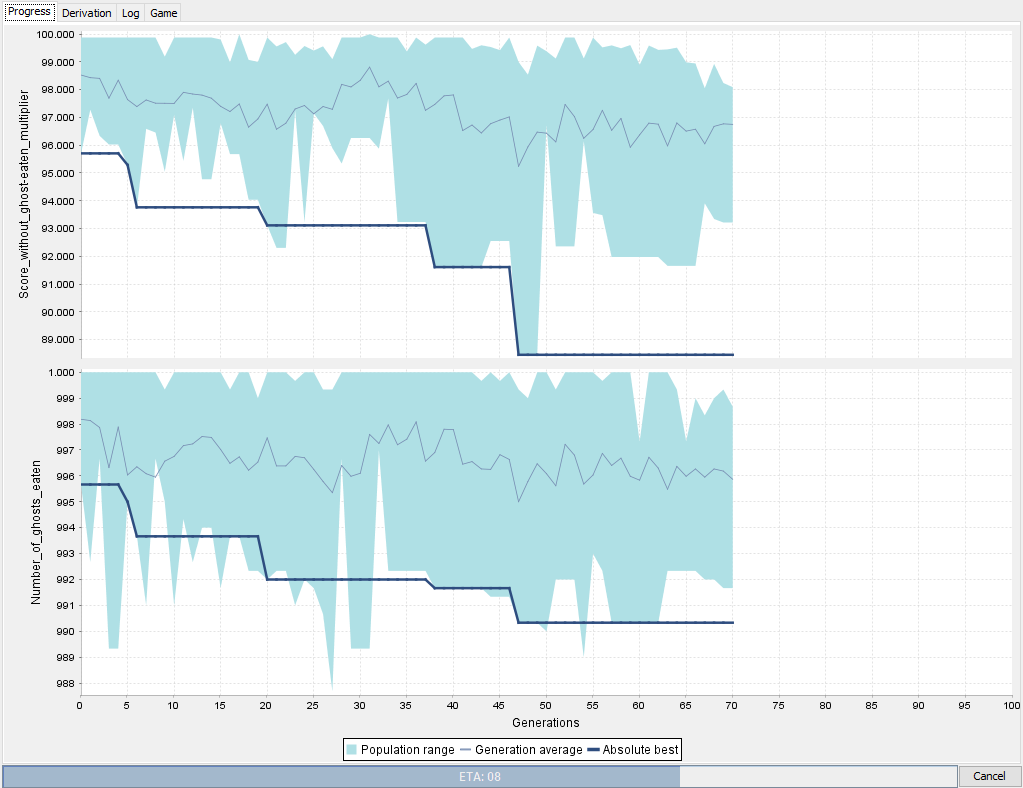
\includegraphics[width=\textwidth]{gui/multi-grafica}
\end{figure}

\subsection{Pestañas}
Tenemos varias presentaciones al mismo nivel, por lo que se han dispuesto diferentes pestañas para cambiar entre ellas. Este diseño no es limitante, permitiendo incluso analizar resultados del entrenamiento anterior mientras se está realizando un nuevo entrenamiento.
\begin{figure}[H]
\centering

\includegraphics[width=7cm]{gui/pestanas}
\end{figure}

\subsection{Tiempo estimado}
Este panel también cuenta con una barra de progreso que aparece durante la ejecución y desaparece al terminar. Indica además el tiempo estimado restante en una etiqueta sobre la barra. Esta barra también cuenta con un botón \textit{Cancel} para detener la ejecución del algoritmo en cualquier punto del entrenamiento, pudiendo hacer análisis de la evolución y ejecuciones del mejor individuo hasta el momento de la parada.
\begin{figure}[H]
\centering

\includegraphics[width=\textwidth]{gui/barra-progreso}
\end{figure}

\section{Panel del mejor individuo}
En cuanto el algoritmo termina de entrenar aquí podemos ver el fenotipo correspondiente al mejor individuo.
\begin{figure}[H]
\centering
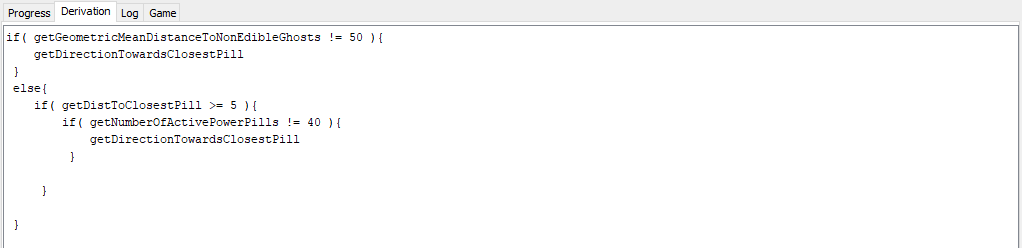
\includegraphics[width=\textwidth]{gui/derivation}
\end{figure}

\section{Panel de juego}
Permite ejecutar y analizar visualmente una partida del juego \textit{Ms. Pac-Man} a partir de un fenotipo dado.

El botón \textit{Copy best here} copia el programa del mejor individuo generado por el algoritmo a la ventana de edición, para después ejecutarlo directamente en Pac-Man con el botón \textit{Run code} o editarlo antes de ejecutar, si se desea.

Los controles contienen además un slider que permite ajustar la velocidad de la partida dentro de un rango razonable.
\begin{figure}[H]
\centering
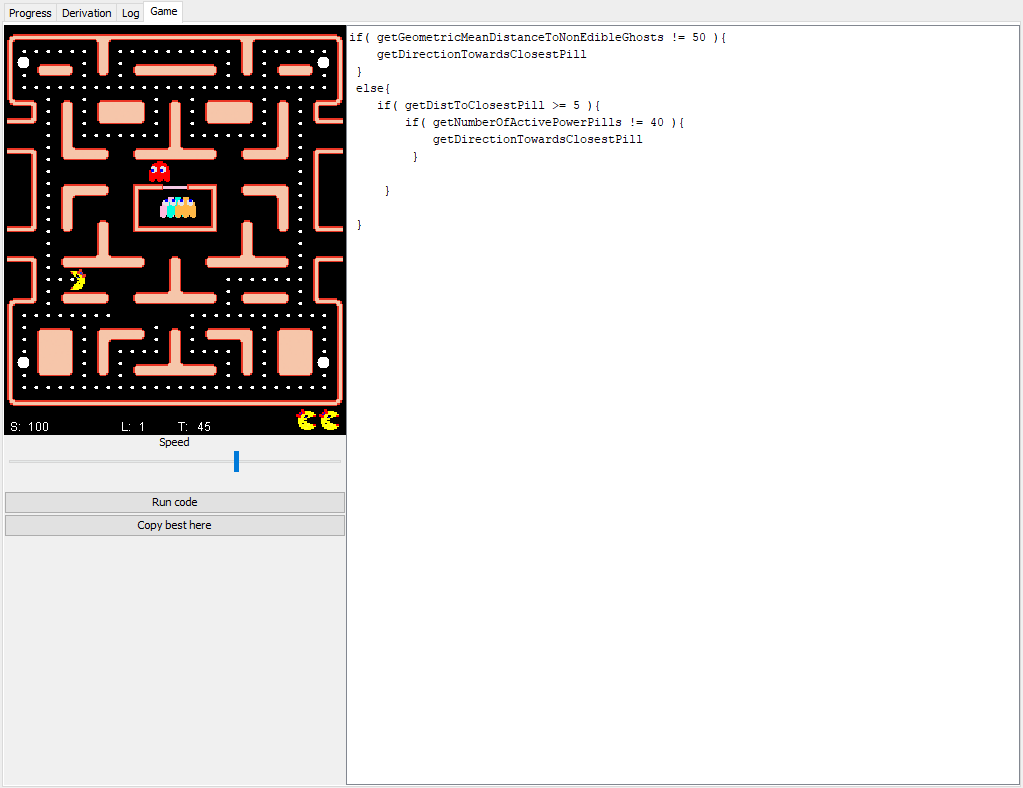
\includegraphics[width=\textwidth]{gui/game}
\end{figure}
